\section{Methodik}

Die methodische Vorgehensweise dieser Arbeit orientiert sich an der Richtlinie 
VDI~2221, welche ein systematisches Vorgehen zur Entwicklung technischer Systeme 
und Produkte beschreibt.\cite{VDI2221, MKon_VL}

Ziel der Richtlinie ist es, den Konstruktionsprozess 
strukturiert, nachvollziehbar und lösungsneutral zu gestalten sowie eine 
reproduzierbare Entscheidungsfindung zu ermöglichen.

Gemäß VDI~2221 erfolgt das Konstruieren nicht als strikt linearer Ablauf, sondern 
als iterativer Prozess. Zwischen den einzelnen Phasen sind Rückkopplungen vorgesehen, 
um neue Erkenntnisse aus späteren Entwicklungsschritten in frühere Phasen 
zurückführen zu können. Dieses iterative Vorgehen ist insbesondere bei komplexen 
technischen Systemen von Bedeutung und wurde auch in der vorliegenden Arbeit 
berücksichtigt.

Für die Entwicklung des automatisierbaren Systems wurden die folgenden 
methodischen Schritte angewendet:

\begin{itemize}
    \item \textbf{Klärung und Präzisierung der Aufgabenstellung}  

    Zu Beginn des Entwicklungsprozesses wurde die Aufgabenstellung analysiert und 
    präzisiert. Dabei wurden die Zielsetzung des Systems, die vorgesehenen Einsatzbedingungen 
    sowie relevante Randbedingungen und Einschränkungen erfasst. Zusätzlich wurde das 
    bestehende System betrachtet, um Schwachstellen, Verbesserungspotenziale und 
    funktionale Zusammenhänge zu identifizieren. Ziel dieser Phase ist gemäß VDI~2221 
    die eindeutige Beschreibung der Entwicklungsaufgabe als verbindliche Grundlage 
    für alle nachfolgenden Schritte.

    \item \textbf{Ermittlung der Anforderungen}  

    Aufbauend auf der geklärten Aufgabenstellung wurden die Anforderungen an das zu 
    entwickelnde System systematisch ermittelt und in einer Anforderungsliste 
    dokumentiert. Diese umfasst sowohl Muss- als auch Wunschanforderungen und 
    berücksichtigt funktionale, geometrische, wirtschaftliche sowie organisatorische 
    Aspekte. Die Anforderungsliste dient während des gesamten Entwicklungsprozesses 
    als zentrales Referenzdokument und bildet die Grundlage für die Bewertung und 
    Auswahl von Lösungsvarianten.

    \item \textbf{Funktionsanalyse}  

    In Anlehnung an die VDI~2221 wurde die Gesamtfunktion des Systems zunächst 
    lösungsneutral betrachtet und anschließend in Teilfunktionen zerlegt. Ziel der 
    Funktionsanalyse ist es, die funktionalen Zusammenhänge innerhalb des Systems 
    transparent darzustellen, ohne sich frühzeitig auf konkrete konstruktive 
    Lösungen festzulegen. Die Funktionsstruktur bildet damit die Basis für die 
    systematische Entwicklung alternativer Lösungsprinzipien.

    \item \textbf{Konzipieren}  

    Auf Grundlage der Funktionsstruktur wurden für die einzelnen Teilfunktionen 
    unterschiedliche Lösungsprinzipien entwickelt. Diese wurden zu mehreren 
    Gesamtkonzepten kombiniert. Zur Bewertung der entwickelten Konzepte wurde eine 
    Nutzwertanalyse durchgeführt. Ziel dieser Analyse war es, die Konzepte anhand 
    mehrerer, aus der Anforderungsliste abgeleiteter Bewertungskriterien systematisch 
    miteinander zu vergleichen und eine nachvollziehbare Entscheidungsgrundlage zu 
    schaffen.

    Die Bewertungskriterien wurden entsprechend ihrer Bedeutung für die 
    Aufgabenstellung gewichtet. Anschließend wurden die einzelnen Konzepte für jedes 
    Kriterium bewertet und die gewichteten Teilnutzen zu einem Gesamtnutzwert 
    zusammengefasst. Das für die weitere Entwicklung herangezogene Konzept wurde auf 
    Basis der Ergebnisse der Nutzwertanalyse ausgewählt.

    \item \textbf{Entwerfen und Ausarbeiten}  

    Das ausgewählte Konzept wurde im weiteren Verlauf schrittweise konstruktiv 
    ausgearbeitet. Dies umfasste unter anderem die Dimensionierung von Bauteilen, die 
    Auswahl geeigneter Norm- und Kaufteile sowie die Auslegung der Schnittstellen 
    zwischen den einzelnen Systemelementen. Entsprechend der VDI~2221 erfolgte dieser 
    Schritt iterativ, sodass Erkenntnisse aus Berechnungen, Simulationen oder 
    konstruktiven Überlegungen zu Anpassungen früherer Entscheidungen führen konnten.
\end{itemize}

Die VDI-2221-Methodik bildet somit den methodischen Rahmen für die Entwicklung des 
automatisierbaren Systems in dieser Arbeit. Durch die strukturierte Vorgehensweise 
wird eine nachvollziehbare und systematische Entwicklung sichergestellt, während 
gleichzeitig ausreichend Flexibilität für iterative Anpassungen erhalten bleibt.

\begin{figure}[htbp]
    \centering
    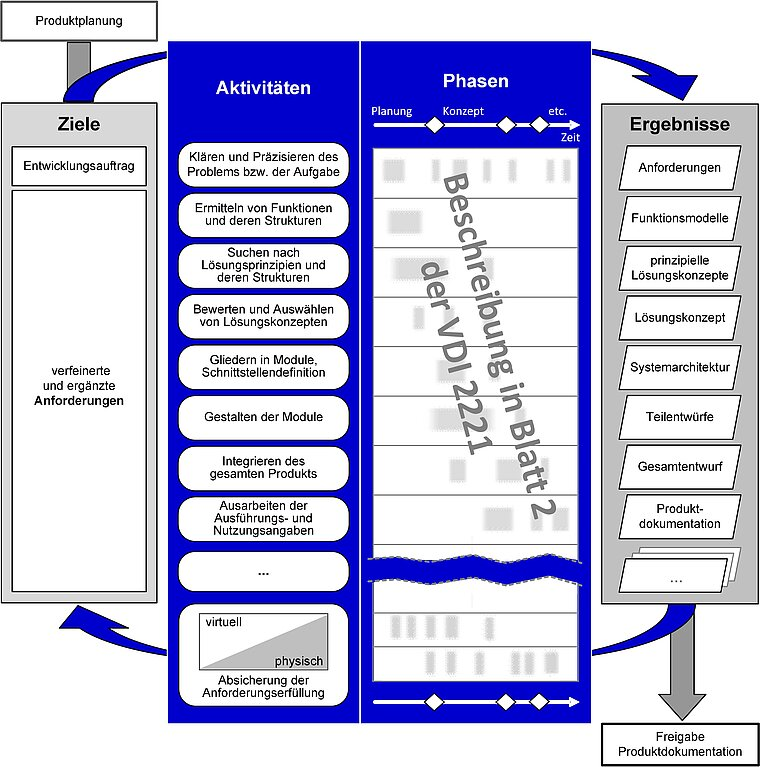
\includegraphics[width=0.8\linewidth]{Bilder/03_Methodik/VDI2221.jpg}
    \caption{Vorgehensmodell der Produktentwicklung nach VDI 2221 (Quelle: VDI 2221) \cite{VDI2221}}
    \label{fig:vdi}
\end{figure}